\RequirePackage{nag}
\documentclass[12pt,letterpaper]{article}
\usepackage{atbegshi}
\usepackage{lipsum}

% \usepackage{fixltx2e}
% \usepackage{classicthesis}
\usepackage{polyglossia}
\usepackage[natbib=true, 
			style=numeric, %authoryear or numeric; comp == compact
			bibstyle=nature, 
			backend=biber,
			uniquelist=false, 
			sorting=none,
			uniquename=false]{biblatex}
\usepackage{booktabs}
\usepackage{relsize}
\usepackage{setspace}
\usepackage{lineno}
\usepackage{wrapfig}
\usepackage{sidecap}

\setdefaultlanguage{english}
\setmainfont[Mapping=tex-text, 
			 Numbers=OldStyle, 
			 % SizeFeatures={{Size=12}}
			 ]{Times}
\setsansfont[Mapping=tex-text, 
			 Numbers=OldStyle, 
			 % SizeFeatures={{Size=12}}
			 ]{Helvetica}
\setmonofont[Scale=0.8]{Monaco}
\setcounter{secnumdepth}{0}

\addbibresource{ELI.bib}

% Set the line spread (height). Be careful here, use too small rather than too
% large value. Also: double-spaced lines correspond to a value of ~1.3,
% depending on the font, NOT to 2.0
\setstretch{1.1} % 1.1 normally

\graphicspath{{figs/}}

%% Custom macros

\newcommand*\captitle[1]{\textbf{#1}}
\newcommand*\todo[1]{%
    \graffito{\textcolor{red}{TO\ DO: #1}}}

\newcommand*\gene[1]{\textit{#1}}
\newcommand*\ko[1]{\textit{#1\textsuperscript{\(-/-\)}}}
\newcommand*\protein[1]{#1}
\newcommand*\species[1]{\textit{#1}}


\title{\ruleline{Project Narrative}}
\lhead{Zhian N. Kamvar, Ph. D.}
\rhead{Project Narrative}

\begin{document}
\maketitle
% \linenumbers

% ------------------------------------------------------------------------------

\section{Training/Career Development Plan}

% The Training/Career Development Plan is a description of all activities that
% the applicant plans to perform and participate to enhance the pre- or
% postdoctoral training during the fellowship award period.

% For Postdoctoral Fellowship applicants, a Training/Career Development Plan
% includes plans for transition to career independence by development of
% professional skills. These professional skills include teaching competencies;
% what those career and training goals are; and results of the postdoctoral
% fellow's previous and current research and scholarships that include
% publications, presentations, etc.
\subsection{Personal Statement}

I am a first year postdoctoral scholar working in the intersection of plant pathology, fungal evolutionary biology, and data science. My Ph. D. dissertation focused on developing open source tools for reproducible analysis of clonal pathogen populations. 
\textbf{My ultimate research goal is to understand how clonal plant pathogen populations evolve in agricultural ecosystems.}
As environmental pressures mount from management practices and changing climate, our food security depends on our knowledge of pathogen evolution \citep{croll2016genetic,grunwald2016population,stukenbrock2013evolution}.
I am also dedicated to the practice of open and reproducible research (Fig. \ref{fig:rr-def}) as there are many well-documented benefits \citep{mckiernan2016open} including the potential for making agricultural science a more diverse and inclusive field.

\begin{wrapfigure}[]{R}[]{0pt}
  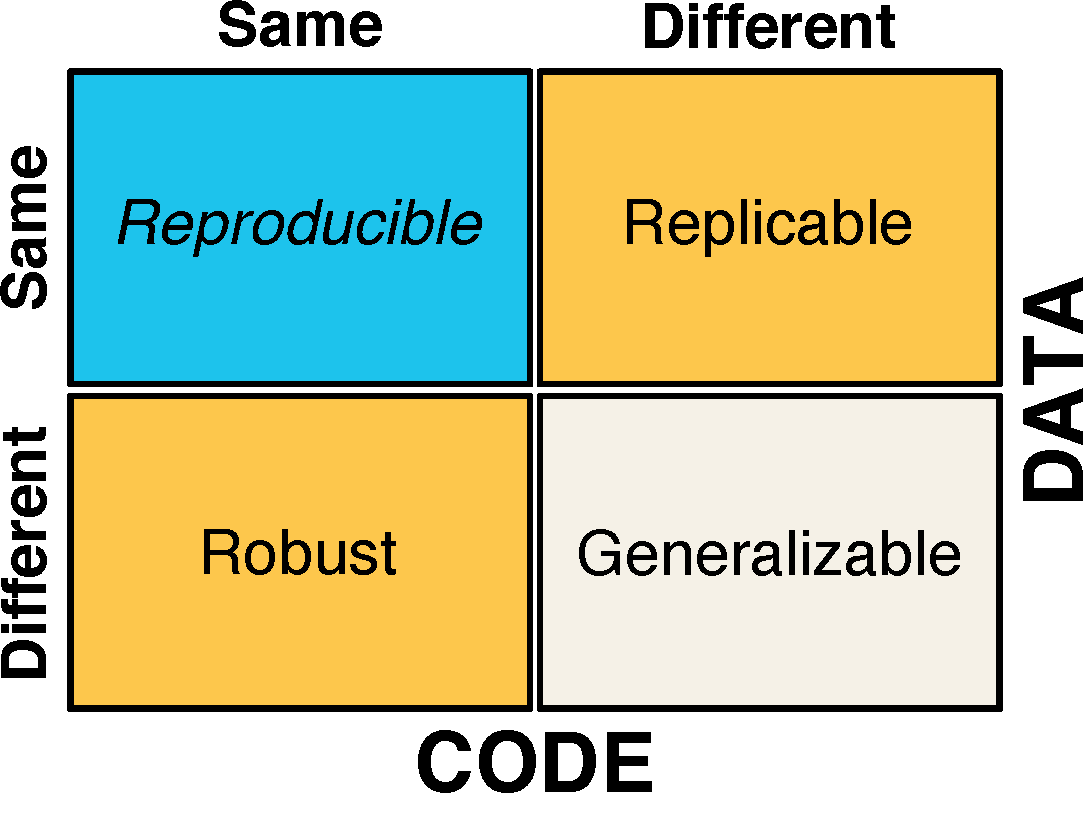
\includegraphics[width=0.35\textwidth]{figure/whitaker2017publishing.pdf}
  \caption{Conceptual definition of computational reproducible research (top left) adapted from \citet{whitaker2017publishing}. If the code and data are the same, they should produce the same results \citep{patil2016statistical}.
  }
  \label{fig:rr-def}
\end{wrapfigure}

Ideally, I would like to pursue this goal by obtaining a faculty position with
research and teaching responsibilities. 
This would place me in a situation where I would be able to contribute to plant pathology by both mentoring the future generation of scientists and pursuing my research interests on the evolution of clonal plant pathogens.
The teacher training that I would receive through this fellowship would both aid in my acquisition of a faculty position and provide a course that I can take
with me in a new position.

The proposed research aims to understand local adaptation of the plant pathogenic fungus \textit{Sclerotinia sclerotiorum} across thermal regions. 
By conducting this research openly, I can use the data and analyses as source materials to create educational activities. 
These will be focused on the topic of reproducible and open research in agricultural sciences, which will be taught as a special topics course in the Department of Plant Pathology at the University of Nebraska-Lincoln. 
A summary of the course will additionally be published in the journal \textit{Plant Health Instructor}. 
\textbf{My overall goals for this fellowship are to develop my skills in education and genomic-scale research.}

When I accomplish these goals, I am confident that I will be adequately prepared to mentor future plant pathologists.

\subsection{Research Training}

Broadly, my current research focuses on understanding the population dynamics and evolutionary processes governing the clonally-reproducing fungal pathogen \textit{S. sclerotiorum}.
I use reproducible research practices for data analysis. 
My research has largely been focused on microsatellite data, and I have experience with genome assembly (i.e. by creating a make-based genome assembly pipeline: \url{https://github.com/zkamvar/read-processing}).
I do not have substantial experience asking evolutionary questions of large-scale genomic data. 
\textbf{The goal of research training} is to compliment my skills as a data scientist with the tools and techniques necessary for evolutionary genomic data analysis. 

\begin{itemize}
  \item \textbf{Background Training In:} population genetics, evolution, molecular techniques, microbiological techniques, and R programming
  \item \textbf{Experienced In:} reproducible research techniques, methods development, cluster computing, population genetic analysis, software development, multivariate analysis, sequence alignment
  \item \textbf{Inexperienced In:} coalescent analysis, Bayesian statistics, phylogeographic analysis
\end{itemize}

\subsubsection*{Research Training Plan}

\begin{enumerate}
  \item \textbf{Workshop on Molecular Evolution at Woods Hole, MA:} this workshop consists of lectures, discussions, and bioinformatic exercises that span contemporary topics in molecular evolution. Training topics specific to my deficiencies include, but are not limited to: phylogenetic analysis (maximum likelihood theory and practice, Bayesian analysis; hypothesis testing), population genetics analysis (coalescence theory, maximum likelihood and Bayesian estimation of population genetic parameters), molecular evolution (gene duplication and divergence, gene family organization), and comparative genomics (genome content, structure, and evolution).
  \item \textbf{Preregistration:} A description of all data, analyses, and expectations will be described in a public preregistration submission to the Open Science Framework (\url{https://osf.io/}).
  \item \textbf{Collection of 96 \textit{S. sclerotiorum} isolates from China and US:} Isolates from four regions in China will be provided by Dr. Weidong Chen; those from four regions in the US will be provided by Dr. James Steadman. 
  \item \textbf{DNA Extraction and Illumina Sequencing:} Genomic DNA will be extracted under the supervision of Dr. Sydney E. Everhart and sent for library preparation and sequencing at the Beijing Genome Institute (BGI). 
  \item \textbf{Data Validation and Analysis:} Genome assembly, data validation,
  and analysis will be done on the Holland Computing Center (HCC) Clusters at University of Nebraska-Lincoln. Genome sequences will be deposited in GenBank and all metadata and analysis scripts will be stored at the Open Science Framework and given a unique Digital Object Identifier.
\end{enumerate}

\subsection{Pedagogical Training}

I have experience teaching short, 3 hour workshops, but do not have formal training in pedagogical methods beyond my training as a Teaching Assistant for a 200 level introductory biology course. 

\begin{itemize}
  \item \textbf{Background Training In:} Assignment evaluation, laboratory section management
  \item \textbf{Experienced In:} Interactive laboratory instruction, K-12 English as a Foreign Language instruction, Short-form workshop development and
  instruction
  \item \textbf{Inexperienced In:} Active learning techniques, course creation and evaluation, developing goals for specific learning outcomes, course portfolio development
\end{itemize}

\subsubsection*{Pedagogical Training Plan}

\begin{enumerate}
  \item \textbf{Workshop training} will be provided by Data Carpentry. In my first year, I aim to complete instructor training and certification.
  \item \textbf{Northstar Summer Institute for Scientific Teaching:} This HHMI-funded program in Twin Cities, MN will cover tools and techniques for scientific teaching. These include modes of assessment, backward design, creating and sustaining inclusive environments, the use of current education literature for course improvement.
  \item \textbf{Course Development:} Development of the reproducible research course will begin immediately by defining public data sets to use as examples and developing basic materials for reproducible research.
  \item \textbf{Special Topics Course in Plant Pathology at UNL:} I will create a three credit-hour special topics course about reproducible research. This will be held in the department of Plant Pathology and offered to anyone in the agricultural sciences. 
\end{enumerate}


\subsection{Career Development}

\begin{itemize}
  \item \textbf{Background Training In:} 
  manuscript preparation, peer-review process, research ethics, outreach methods
  \item \textbf{Experienced In:} 
  professional writing (CV, r\'esum\'e, cover letters), written and oral communication of scientific research to professional and lay audiences, leadership
  \item \textbf{Inexperienced In:} research grant writing, course development, grant budget management, inter-organizational leadership
\end{itemize}

\subsection{Career Development Plan}

% Might want to include mentoring of graduate and undergraduate students as part
% of your career development plan.
\begin{enumerate}
  \item \textbf{Professional Development} in writing grant proposals, and grant-budget management will be provided under the guidance of Dr. Sydney E. Everhart.
  \item \textbf{Develop five-year plan} for future projects, funding sources, and jobs including applications to tenure-track faculty positions.  
\end{enumerate}

% ------------------------------------------------------------------------------


\section{Mentoring Plan}

The goal of this proposed integrated project is to provide the fellow with teaching and analytical skill sets that will enable a transition into an independent research and teaching career. 
Training will be received in three ways: 1) through the teaching and molecular biology workshops as described in the above section 2) through formal monthly evaluation of progress reports, and 3) through informal meetings as needed by the fellow. 
The monthly meetings will ensure that the fellow is held accountable for all project deliverables (Fig. \ref{fig:timeline}). 
Both mentors have committed to work closely with the fellow on this project.

The primary mentor, Dr. Sydney E. Everhart, will provide mentoring in all research and career development aspects of this project.
The collaborating mentor, Dr. Jenny Dauer, will provide mentoring in the development for the pedagogical skill set.
The fellow will be evaluated on organization and completion of project deliverables as well as adaptation to any unforseen pitfalls. 



% \noindent The applicants are expected to engage their mentors and/or advisors in the
% development of their application. Thus, prior to submission of the
% application, prospective fellows should already identify a Primary mentor who
% will be willing to help them in their projects as well as professional
% development (note: more than one Primary Mentor is acceptable for Integrated
% Projects Only). If there are other collaborating mentors, their role and
% responsibilities to the project and development of the applicant's skills
% should be clearly described. Because this is a
% very important component of the project, the commitment of the mentor(s) is
% included in the evaluation criteria as it pertains to project personnel. In
% describing the role of the mentor, the applicant should:

% \begin{enumerate}

%   \item Briefly indicate how the mentoring and educational training will add to the
%    skill sets of the National Institute of Food and Agriculture (NIFA) Fellow.

%   \item Briefly explain the commitment of the primary mentor.

%   \item Briefly describe the role of collaborating mentors (if applicable).

%   \item With respect to the Primary Mentor, provide a list of former mentees and
%    their current positions. 
%    \begin{quote}
%    NOTE: The Primary Mentor shall submit a Letter of Commitment (as an
%    attachment to Field 12, Other Attachments, of the Other Project
%    Information form-see section g. in the AFRI ELI RFA) explicitly
%    indicating their respective responsibilities throughout the proposed
%    project in relation to the Project Director.
%    \end{quote}

%   \item Briefly list and explain the role of other non-primary mentors.

% \end{enumerate}

\noindent \textbf{Mentor's Former Mentees and their current positions}


% \begin{tabular}{p{0.25\linewidth}p{0.2\linewidth}p{0.4\linewidth}}
% \textbf{Name} & \textbf{Position} & \textbf{Current} \\
% \hline\\
% Thomas Miorini & postdoc & postdoctoral scholar with Dr. Loren Giesler, Department of Plant Pathology, UNL\\

% B. Sajeewa Amaradasa & postdoc & postdoctoral scholar with Dr. Nick Dufault, Department of Plant Pathology, University of Florida\\

% Sarah Campbell & undergrad assistant & graduate student with Drs. Phil Brannen and Harald Scherm, Department of Plant Pathology, University of Georgia\\

% Morgan Thompsen & undergrad assistant & working towards completion of her bachelor's degree in biological science for pre-nursing, UNL\\

% Josh Hanson & undergrad assistant &working towards completion of his bachelor's in Biological Systems Engineering, UNL\\
% \hline
% \end{tabular}

\begin{itemize}
  \item Thomas Miorini, postdoctoral scholar UNL 2016-2017; presently postdoctoral scholar with Dr. Loren Giesler, Department of Plant Pathology, UNL

  \item Bimal Sajeewa Amaradasa, postdoctoral scholar UNL 2014-2016; presently postdoctoral scholar with Dr. Nick Dufault, Department of Plant Pathology, University of Florida

  \item Sarah Campbell, undergraduate lab assistant UNL 2014-2016; presently graduate student with Drs. Phil Brannen and Harald Scherm, Dept. of Plant Pathology, University of Georgia

  \item Morgan Thompsen, undergraduate lab assistant UNL 2016; presently working towards completion of her bachelor's degree in biological science for pre-nursing, UNL

  \item Josh Hanson, undergraduate lab assistant UNL 2014-2016; presently working towards completion of his bachelor's in Biological Systems Engineering, UNL
\end{itemize}


% ------------------------------------------------------------------------------

\section{Project Plan}

\subsection{Introduction}

\begin{wrapfigure}[29]{R}[]{0pt} % 8 if hanging on new page
  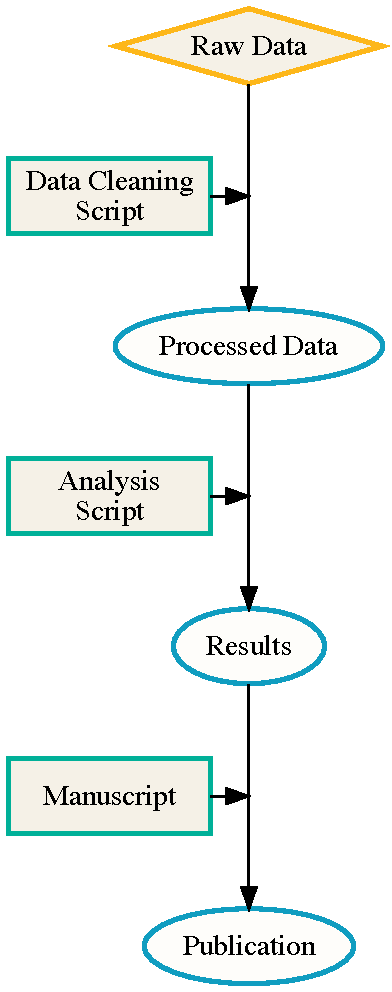
\includegraphics[width=0.275\textwidth]{figure/rr.pdf}
  \caption{Diagram of an automated reproducible research workflow}
  \label{fig:rr}
\end{wrapfigure}

Principles behind the concept of reproducible research suggest that if a researcher can recreate the results of another individual's study using the same data and analyses, then it is reproducible (Fig. \ref{fig:rr-def}) \citep{buckheit1995wavelab,peng2011reproducible,patil2016statistical}. 
In theory, all scientific research should be reproducible, but in practice, this is not always the case.
A recent survey revealed that up to 50\% of researchers were unable to reproduce their own published results and that 90\% indicated that there was a ``reproducibility crisis'' \citep{baker2016scientists}.
Despite major journals and funding agencies taking steps to implement incentives for transparency \citep{nature2017announcement}, \textbf{there is still a need for training on reproducibility across the biological science disciplines} \citep{barone2017unmet}.
In the last decade, computational tools have become available that make reproducibility more accessible \citep{boettiger2015introduction,wilson2016good}.
Moreover, there are many benefits for scientists who adopt open and reproducible methods including increased citation counts, a greater chance of receiving external funding, and improved relationships among peers potential collaborators \citep{mckiernan2016open,stewart-lowndes2017path,schmidt2016stepping}.

The results produced from agricultural sciences research often have a direct effect on key agricultural stakeholders. 
As a result, it imperative that research results be replicable. 
As genomic and microbiome data becomes more readily available, scientists with very little background in bioinformatics are conducting studies with no knowledge of how to process their data \citep{stewart-lowndes2017path, barone2017unmet}. 
To address the need for training on reproducible research and bioinformatics, \textbf{the long term goals} of the proposed project are to: \textbf{a)} develop a course on reproducible research for students in agricultural sciences using real-world examples and \textbf{b)} create an open and reproducible example of genomic research. The second part will be carried out by testing the \textbf{hypothesis} that, due to increased generational times, the plant pathogenic fungus, \textit{Sclerotinia sclerotiorum} is locally adapted to subtropical climates.
To complete these goals and test this hypothesis, we seek completion of the following \textbf{objectives}:
\begin{itemize}
  \item \textbf{Objective \#1:} Create educational materials for graduate students using agricultural data, covering topics from data validation and curation, method choice, version control, and open data science practices (Fig. \ref{fig:rr-def}, \ref{fig:rr}).
  \item \textbf{Objective \#2:} Perform whole genome sequencing on 96 isolates of \textit{S. sclerotiorum} collected hierarchically over eight subpopulations across North America and East Asia (Fig. \ref{fig:us-china}).
  \item \textbf{Objective \#3:} Perform population genetic, phylogeographic, and coalescent analyses to detect and test signatures of local adaptation to climate regions.
  \item \textbf{Objective \#4:} Lead a semester-long special topics course on reproducible research in the department of Plant Pathology at the University of Nebraska-Lincoln.
\end{itemize}

\begin{SCfigure}[][h!]
  \centering
  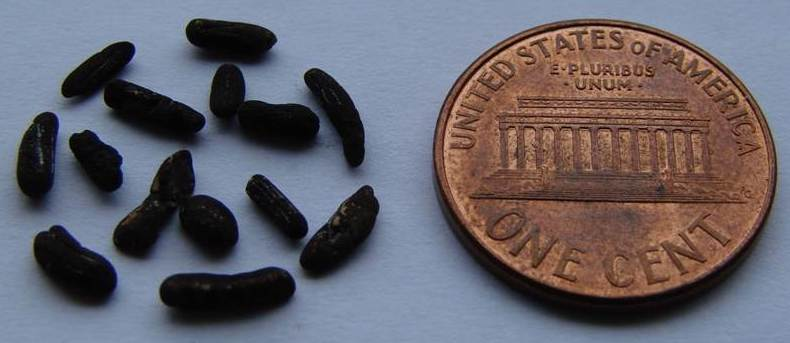
\includegraphics[width=0.5\textwidth]{figure/sclerotia.jpg}
  \caption{Sclerotia of \textit{S. sclerotiorum} (left). Sclerotia can germinate producing apothecia. Ascospores from apothecia serve as primary inoculum. Image and description modified from L. Del Rio Mendoza (\url{https://www.ag.ndsu.edu/sclerotinia/pictures.html})}
  \label{fig:sclerotia}
\end{SCfigure}

\subsubsection*{Need For Proposed Project}

\textit{Sclerotinia sclerotiorum} (Ascomycota) is a cosmopolitan, haploid, plant pathogenic soil fungus with over 400 hosts worldwide \citep{bolton2006sclerotinia} and causes up to \$252M in losses per year on sunflower, soybeans, dry edible beans, canola, and pulse crops \citep{uscanola}.
Reproduction is largely asexual, but outcrossing has been known to occur \citep{bolton2006sclerotinia,attanayake2014inferring}. 
This fungus can survive for several years in the soil in the form of melanized sclerotia (Fig. \ref{fig:sclerotia}) \citep{bolton2006sclerotinia}.
Due to its wide host range and necrotrophism, management of this pathogen largely involves fungicide applications and, to a lesser extent, resistant cultivars \citep{bolton2006sclerotinia}.
Effective management strategies for any fungal pathogen depends on the knowledge of genetic diversity and adaptive potential \citep{grunwald2016population}. 

Studies using both phenotypic traits and molecular markers have suggested that \textit{S. sclerotiorum} may be locally adapted to thermal conditions \citep{huang1991temperature,carbone2001microbial}.
Numerous studies over the last 30 years around the world show increased diversity in subtropical regions, but \citet{lehner2017sclerotinia} show that this may be an artifact of low-resolution genetic markers.
In the past 30 years, studies have been conducted either across continental or climate regions, but no studies have addressed if the differences observed between \textit{S. sclerotiorum} populations is due to climate or region.
In addition, no previous studies have evaluated the population genomic variation of this fungal pathogen, despite more than 50 population studies to date using SSR markers, which have been shown to poorly resolve haplotype diversity \citep{lehner2017independently}. 

% Might want to emphasize that no previous studies have evaluated the population
% genomic variation of this fungal plant pathogen, despite XX number of
% population studies to date using SSR markers.

As \textit{S. sclerotiorum} occurs globally, it is important to determine if populations are adapted to thermal gradients, which could affect dispersal under warming climate conditions \citep{bolton2006sclerotinia,lehner2017sclerotinia,croll2016genetic}.
Significant levels of differentiation have been found between populations on canola in the United States (US) and China \citep{attanayake2013sclerotinia}, but these populations occur in different climate regions.
To test the hypothesis of local adaptation to thermal environments, we plan to infer genetic diversity, and migration patterns with modern, reproducible population genetic and phylogeographic approaches on whole genome sequence data. 


\subsection{Rationale and Significance}


\noindent
\textbf{AFRI Foundational Priority for Plant Health and Production and Plant Products}

The rationale of the proposed work is that 
\textbf{1)} producing educational materials on open and reproducible research will have long-term benefits for agricultural research by increasing access to education and emphasizing practices that will positively influence stakeholder confidence, 
\textbf{2)} the identification of patterns for adaptation in \textit{S. sclerotiorum} will reduce inputs by influencing management decisions regarding movement of inoculum, and 
\textbf{3)} genomic data and analyses from 96 isolates of \textit{S. sclerotiorum} will help drive novel research on this cosmopolitan pathogen. 

The practice of open and reproducible research has been shown to increase the speed and accuracy of which scientific research is conducted \citep{stewart-lowndes2017path, wilson2016good}.
Surveys conducted in 2016 showed that 90\% of researchers acknowledge a reproducibility crisis in science \citep{baker2016scientists} and that the most pressing need is for training on data management and integration \citep{barone2017unmet}. 
Major scientific journals have even implemented checklists \citep{nature2017announcement} and badges \citep{kidwell2016badges} in an effort to incentivize reproducibility.
Calls for conscious efforts to increase reproducibility have been around for many years \citep{buckheit1995wavelab, peng2011reproducible}, but only recently has training been emphasized \citep{schmidt2016stepping, stewart-lowndes2017path, wilson2016good}. 
By training graduate students seeking masters or doctoral degrees on how to perform open and reproducible research, future agricultural science will be cost effective, innovative, and engaging. 
This is in line with the teaching mission of the University of Nebraska, where multidisciplinary graduate education is explicitly mentioned as a focal point.

Canola production is a growing industry in the United States, producing three billion pounds of seed grossing at \$500 million in 2016 \citep{usda2017production, usda2017values}. Losses due to Sclerotinia Stem Rot are estimated to be one percent yield for every two percent disease incidence \citep{delrio2007impact}, and the midwest has seen an average incidence rate of 13\% \citep{markell2009sclerotinia}, which would mean an annual loss of \$30 million. 
It is known that local climate can exacerbate the spread of inoculum and thus, understanding the evolutionary potential for \textit{S. sclerotiorum} to adapt to a warming climate is essential for targeting future management decisions \citep{attanayake2014inferring,shea2000integrated,billiard2012sex}.

For over 15 years, population genetic analysis on \textit{S. sclerotiorum} has been performed using the same set of simple sequence repeat (SSR) markers \citep{sirjusingh2001characterization}. 
These markers, however, have been unable to accurately determine the number of unique genotypes in a sample \citep{lehner2017independently, lehner2017sclerotinia,arnaud2007standardizing}.
Moreover, these markers may suffer from confirmation bias, only able to describe the diversity of \textit{S. sclerotiorum} in the Midwestern United States \citep{attanayake2013sclerotinia}. 
Using whole genome sequences of representative isolates across continents allows us to capture a breadth of diversity, giving us a clear picture of the adaptive potential in \textit{S. sclerotiorum} \citep{grunwald2016population}.
By understanding the potential for thermal adaptation in \textit{S. sclerotiorum}, we can better predict how it will respond to changes in climate \citep{croll2016genetic}.


\subsection{Approach}


\subsubsection*{Objective \#1: Development of Education Modules}

The overall goal of the course is to help students develop thought processes that allow them to adapt to new tools and workflows. 
The objective of the course is for the students to be able to identify and utilize reproducible research practices including data management, version control, scripting, and archiving with the Open Science Framework (\url{https://osf.io/}).
The target audience for this course are graduate students in the agricultural sciences.

\noindent \textbf{Methods -} 
The fellow will use a combination of materials previously developed for other domains of research (i.e. \url{http://kbroman.org/Tools4RR/}) and small example data sets (i.e. those found in \citet{sparks2008ecology}) for development of primary course materials. 
This course will be split up into four distinct sections, Philosophy of Open Science, Data Management and Ethics, Best Practices in Reproducible Research, and Research Dissemination.
The students will be encouraged to use their own data or choose a publicly available data set (i.e. from \url{https://www.data.gov/}) to ask questions and test their own hypotheses.
The course will be taught using the R programming language, but knowledge of the language will not be required \citep{R2017}.
All course materials with a website will be publicly available on GitHub and archived on the CERN-funded Zenodo (\url{https://zenodo.org/}).\\
\noindent \textbf{Expectations -}
By the end of the first year, the fellow expects to have a publicly available, fully developed course on reproducible research.
This work will be licensed in the public domain, allowing other educators to freely use this material in their own courses.\\
\noindent \textbf{Pitfalls and Limitations -}
GitHub currently allows open source projects to be hosted free of charge, but since they are a for-profit company, their policy could change at any time. If this risk presents itself, the data are archived at Zenodo and the fellow will host the materials on the Open Science Framework.

\subsubsection*{Objective \#2: Whole Genome Sequencing of 96 \textit{Sclerotinia sclerotiorum} Isolates}

\begin{wrapfigure}[16]{l}[]{0pt} % [lineheight]{position}[overhang]{width}
  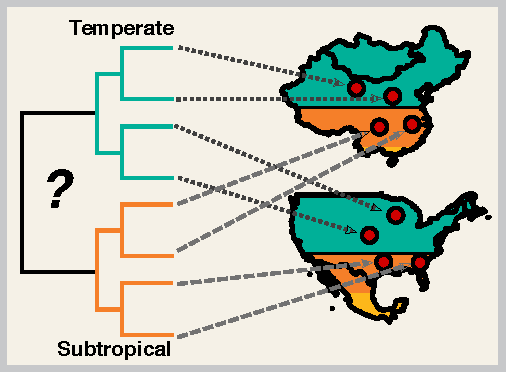
\includegraphics[width=0.35\textwidth]{figure/us-china.pdf}
  \caption{A hypothesis of the evolutionary history of \textit{S. slcerotiorum} in temparate and subtropical regions between North America and East Asia}
  \label{fig:us-china}
\end{wrapfigure}
\noindent \textbf{Sampling and Experimental Design -}
A total of 96 isolates split evenly across eight subpopulations of \textit{S. sclerotiorum} will be gathered from canola fields in China and the USA representing temperate regions temperate regions (between $40^{\circ}N$ and $66^{\circ}N$) and subtropical regions (between $23.5^{\circ}N$ and $40^{\circ}N$) (Fig. \ref{fig:us-china}).
Isolates from China will be random samples from Gansu, Qinghai, Anhui, and Hunan provinces originating from \citet{zhou2014dimethachlon} and \citet{attanayake2013sclerotinia}.
Isolates from USA will be from canola fields in North Dakota, Colorado, Georgia, and South Carolina \citep{aldrich-wolfe2015genetic,phillips2002phylogeography}.
Prior to DNA extraction, all isolates will be grown on Potato Dextrose Agar (PDA) for 5 days at $24^{\circ}C$ and transferring four 8mm plugs to an 100mL liquid PDA with shaking for four days at $24^{\circ}C$ as performed in \citet{derbyshire2017complete}.\\
\noindent \textbf{DNA Extraction -}
Mycelia will be collected via vacuum filtration, discarding agar plugs. Tissue will be homogenized using liquid nitrogen in sterile mortar and pestles stored $-80^{\circ}C$. Extraction will be performed using the DNA Plant Maxi Kit (Qiagen) following manufacturer's instructions yielding into 1mL sterile Milli-Q Water (Millipore). Final DNA concentration will be checked using the Qubit Fluorametric quantification system (ThermoFisher) and quality will be assessed via 1\% gel electrophoresis. DNA will be stored at $-80^{\circ}C$.\\
\noindent \textbf{Genome Sequencing and Alignment -} 
Whole genomic DNA will be sent to the Beijing Genomics Institute (BGI) for Illumina (Illumina inc.) library preparation of 150bp paired-end libraries and sequencing. Libraries will be sequenced to $>15\times$ depth with samples from all populations evenly split on two lanes of Illumina HiSeq 4000 sequencer.
Data will be downloaded from BGI, validated by checking the MD5 hash sums, and read-only copies will be uploaded to UNL's Attic storage system and the Open Science Framework. 
On UNL's cluster computing infrastructure, reads will be mapped to the \textit{S. sclerotiorum} reference genome using a workflow modified from \url{https://github.com/zkamvar/read-processing}, which uses \textsc{Bowtie2} and \textsc{Samtools} to map reads and \textsc{GATK} for variant discovery \citep{langmead2012fast, li2009sequence, mckenna2010genome, derbyshire2017complete}.\\ 
\noindent \textbf{Expectations -}
Based on preliminary results from sequencing clonal strains of \textit{S. sclerotiorum} after fungicide exposure we expect to see, on average, $\geq98.5\%$ coverage with $\geq8\times$ depth for all isolates. Because the reference genome of \textit{S. sclerotiorum} is from the US, we additionally expect a greater number of variants in the isolates from China.\\
\noindent \textbf{Pitfalls and Limitations -}
If the differentiation due to continent is sufficiently large, our alignments of the isolates from China may not efficiently align to the reference genome. 
We can monitor this by assessing mapping quality for all alignments and performing de-novo assembly on the isolates.

\subsubsection*{Objective \#3: Assessment of Local Adaptation to Climate}

\noindent \textbf{Methods -} 
We will use phylogenetic data from each gene independently to assess the evolutionary history of these populations using \textit{Botrytis cinerea} as an outgroup \citep{staats2012genome}. 
To address phylogenetic incongruence, we will use newly developed multivariate methods for exploring the space of phylogenetic trees across the genome \citep{kendall2016mapping, jombart2017treespace}. 
Adaptive potential will be assessed using ratios of synonymous and non-synonymous mutation rates, classifying them into positive, neutral, or negative selection, and comparing them to classes of tree topologies (geo-centric, climate-centric, or random) via $\chi^2$ test.
Migration rates between populations will be assess using Approximate Bayesian Computation with coalescent simulations. 
To assess migration among climate and geographic regions, we will use \textsc{ABCtoolbox} \citep{wegmann2010abctoolbox}. 
Simulations will be carried out on each gene independently using the \texttt{msprime} simulator \citep{kelleher2016efficient}. 
Mean nucleotide diversity ($\pi$) and mean number of alleles will be used as summary statistics for evaluating simulations. 
Partial least squares regression and Euclidean distance to observed data will be utilized as the rejection method.\\
\noindent \textbf{Expectations -}
Based on initial data from \citet{attanayake2013sclerotinia}, I expect a majority of genes will segregate for geographic differentiation, but I predict that the majority of the positive selection will be found in the climate-centric genes, whereas the others will be majority neutral.\\
\noindent \textbf{Pitfalls and Limitations -}
If the samples are not true representatives of their populations, there exists a possibility for false positives for a signature of adaptation to climate.

\subsubsection*{Objective \#4: Leading and Evaluating Special Topics Course}

In the beginning of the second year, a special topics course will be offered in the Plant Pathology Department at UNL targeted at graduate students in the agricultural sciences.

\noindent \textbf{Methods -}
The course duration will be one full semester. 
Course instruction will be designed using an active learning approach \citep{freeman2014active}.
A strict code of conduct emphasizing inclusiveness, accessibility, and anti-harassment will be enforced.
Lecture will be interspersed with short discussion sections and knowledge-based quizzes.
Students will be expected to identify a project using their own data or data sets found in public repositories (i.e. \url{https://www.usda.gov/content/usda-open-data-catalog}) in the first three weeks of the course.
To emphasize the importance of communication, the students will be asked to tailor final reports of their projects to a specific audience.
Evaluation will be based on participation, in class quizzes, and the successful execution of the final project.
Upon completion of the course, a description will be written and submitted to the peer-reviewed publication \textit{The Plant Health Instructor}.\\
\noindent \textbf{Expectations -}
Each student will have a completed project that is fully reproducible. 
Because of the emphasis on open science, we also expect at least half of the projects to be openly available.
The training in reproducible research and communication has the long-term benefits of advancing scientific progress at a faster rate due in part due to verifiable workflows and increased confidence in communication.\\
\noindent \textbf{Pitfalls and Limitations -}
The students will be self-selecting for those interested in reproducible research and open science.
To avoid this, advertisements will be tailored to specific departments and will emphasize that no prior knowledge of reproducible research is required.

\noindent \textbf{Hazards -} No known hazards are associated with this project.\\
\noindent \textbf{Timeline -} The proposed objectives will be completed within the timeline presented in Figure \ref{fig:timeline}.

\begin{figure}[!htbp]
  \centering
  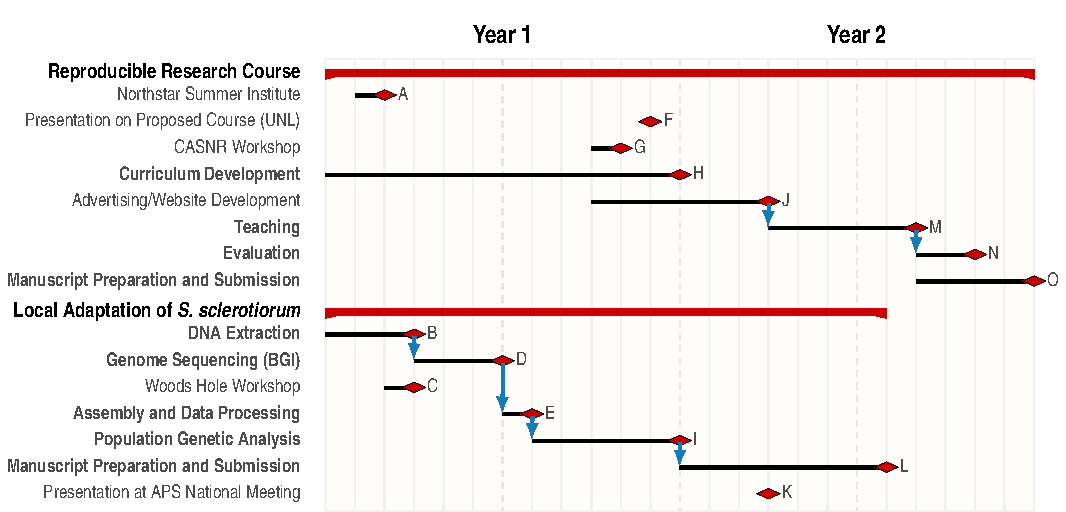
\includegraphics[width=0.95\textwidth]{packet/timeline.pdf}
  \caption{Project Timeline. The milestones \textbf{A-N} each represent generation of a measurable outcome used in the evaluation plan.}
  \label{fig:timeline}
\end{figure}


% ------------------------------------------------------------------------------

\section{Evaluation Plan}

\subsection{Progress Evaluation}

Monthly progress reports will be written and shared with mentors identifying achieved, in-progress, and outstanding goals as well as challenges and opportunities. During the first year, a quarterly course curriculum update and evaluation will be presented to the project mentors in group meetings. Course progress will be assessed by monthly observations from the project mentors and anonymous surveys from the students. 

\subsubsection*{Milestones}
\begin{itemize}
  \item \textbf{6 months:} Genomes sequenced (\textbf{B, D}), workshops on teaching and molecular evolution attended (\textbf{A, C}), outline for each week of course created, preregistration of research uploaded to the Open Science Framework
  \item \textbf{12 months:} Genomes assembled (\textbf{E}), population genetic analysis performed (\textbf{H}), lesson plans for each week of the course completed (\textbf{G}), special topics course registered, course website created, presentation at UNL Plant Pathology Seminar held (\textbf{F}).
  \item \textbf{18 months:} Presentation at APS National Meeting on research (\textbf{J}), course for graduate students underway
  \item \textbf{24 months:} Course completed (\textbf{I, L, M}), materials freely available in the public domain, manuscripts submitted as preprints to the Open Science Framework (\url{https://osf.io/preprints/}) and to both \textit{Molecular Ecology} and \textit{Plant Health Instructor} (\textbf{K, N}).
\end{itemize}

\subsection{Dissemination Plan}

\noindent \textbf{Research Data and Scripts} will be deposited in the Open Science Framework. All materials will be released with open licenses. Data will be released under the ODC Open Database License 1.0 and code will be released under the MIT License. \\
\noindent \textbf{Course Materials} will be hosted on GitHub and archived on Zenodo. To promote sharing and reuse, all applicable materials will be released in the public domain. \\
\noindent \textbf{Publications} will first be submitted as preprints to the Open Science Framework preprint server. They will additionally be submitted for peer-review in the journals \textit{Molecular Ecology} and \textit{Plant Heath Instructor}. \\
\noindent \textbf{Presentations} will be held in both UNL and the American Phytopathological Society (APS) National Meeting. The presentation at UNL will be focused on the benefits of reproducible research and open science. The presentation at the APS National Meeting will be on my research on \textit{S. sclerotiorum}.
% ------------------------------------------------------------------------------


% https://tex.stackexchange.com/a/224803/77699
\newpage
\AtBeginShipout{%
\AtBeginShipoutDiscard
}

\printbibliography

\end{document}
